\documentclass[11pt]{article}
\usepackage{techcon_LaTeX_style_v4}
\usepackage{graphicx}
\usepackage{booktabs}
\usepackage{amsmath}
\usepackage{url}

% COVER PAGE ONLY: replace these three fields before submission.
\title{CAP-MF: Empirically Grounded Interaction-Aware Scheduling for Energy-Efficient LLM Inference}
\author{[AUTHOR NAME(S)] \\
[BUSINESS UNIT(S)] \\
[FULL HPE EMAIL ADDRESS(ES)]}

% Reproducibility fields. Populate only from the retained environment manifest.
\newcommand{\vllmversion}{[INSERT FROM MANIFEST]}
\newcommand{\torchversion}{[INSERT FROM MANIFEST]}
\newcommand{\cudaversion}{[INSERT FROM MANIFEST]}
\newcommand{\driverversion}{[INSERT FROM MANIFEST]}
\newcommand{\modelrevision}{[INSERT RESOLVED MODEL COMMIT SHA]}

\begin{document}
\tccoverpage

% Technical pages begin here. No author-identifying information below.
\tctitle{CAP-MF: Empirically Grounded Interaction-Aware Scheduling for Energy-Efficient LLM Inference}

\tcabstract{
Large language model (LLM) requests vary in input length, output length, energy cost, and interference when colocated. Placement based only on isolated measurements can therefore waste accelerator energy, while Exact interaction-aware assignment becomes combinatorial. We present CAP-MF, a capacity-projected Mean-Field scheduler grounded in measured vLLM energy, latency, and directional pairwise interference. Across ten chronological 16-request BurstGPT windows, CAP-MF achieved a 0.00073\% mean optimality gap and a 0.00729\% maximum gap relative to Exact, compared with 2.93\% and 7.05\% for Greedy. CAP-MF converged in every window. In five-repeat live vLLM replay, CAP-MF matched Exact within 0.05\% measured GPU energy and reduced energy per request by 15.54\% relative to Greedy, with 2.93\% higher mean latency and 3.34\% lower virtual request throughput.
}

\section*{Problem statement}
Enterprise LLM services must assign heterogeneous requests while balancing accelerator energy, latency, throughput, and capacity. vLLM improves request execution through PagedAttention and efficient KV-cache management \cite{ref:vllm}, but configuration-level assignment remains a separate problem. A request's cost depends not only on its isolated profile but also on the other requests sharing a serving replica. Our measurements show non-uniform and directional effects: request class $i$ can be strongly affected by class $j$ even when the reverse effect is small. Independent placement can therefore increase energy or latency. For HPE, an interaction-aware scheduler can reduce cost per inference and the energy footprint of enterprise AI infrastructure while making performance trade-offs explicit.

\section*{Our solution}
We profile nine input/output-length classes, $\{SS,SM,SL,MS,MM,ML,LS,LM,LL\}$, on one-GPU TP1 and two-GPU TP2 vLLM configurations. Directional interference is measured as
\[
J_{ij}(c)=L_i^{ij}(c)/L_i^{solo}(c)-1,
\]
where $L_i^{ij}$ is the latency experienced by class $i$ when paired with class $j$ on configuration $c$. CAP-MF approximates the coupled assignment distribution with request probabilities $q_i(c)$. Its local field retains measured directionality:
\[
h_i(c)=E_i(c)+\lambda\sum_{j\ne i}q_j(c)J_{ij}(c),\qquad
\widehat q_i(c)\propto\exp[-h_i(c)/\tau].
\]
Mean-Field methods replace a coupled distribution with a tractable factorized approximation \cite{ref:meanfield}. A discontinuous overload penalty oscillated when demand exactly matched capacity. CAP-MF instead projects every update onto
\[
\sum_c q_i(c)=1,\quad q_i(c)\ge0,\quad \sum_iq_i(c)\le C_c,
\]
then performs capacity-aware hard recovery. Exact integer optimization provides a small-instance oracle; Greedy provides a low-overhead baseline.

\begin{figure}[ht]
\centering
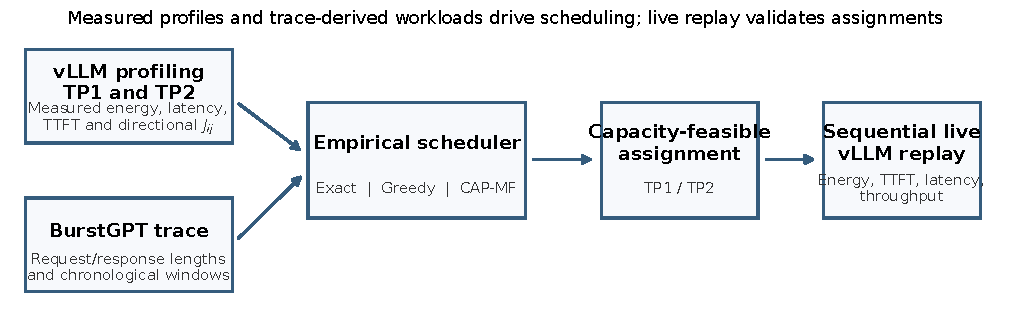
\includegraphics[width=0.98\columnwidth]{fig1_architecture.pdf}
\caption{Empirical profiling, trace-driven assignment, and sequential live replay. TP1 and TP2 are physically measured; any N=32 extension uses replicated logical configurations parameterized from these measurements, not a physical four-replica deployment.}
\label{fig:architecture}
\end{figure}

\section*{Evidence the solution works}
\textbf{Testbed and trace.} We evaluated Qwen2.5-1.5B-Instruct in FP16 on two NVIDIA T4 GPUs using vLLM \vllmversion, PyTorch \torchversion, CUDA \cudaversion, NVIDIA driver \driverversion, and model revision \texttt{\modelrevision}. These values must be inserted from the retained environment manifest before submission. We measured isolated energy and latency for nine classes and all $9\times9$ directed pairs on TP1 and TP2, yielding 162 pair conditions. Maximum observed pairwise latency degradation was approximately 12\%. TP2 provided negligible mean isolated-latency improvement for this model while consuming approximately 17\% more energy on average.

BurstGPT contains real request and response lengths from Azure OpenAI services and was created to address unrealistic LLM-serving workloads \cite{ref:burstgpt}. From 10,000 trace rows, 9,229 valid requests remained. We retained 3,716 requests (40.26\%) within 50\% of a directly measured token-length operating point. We excluded the remainder rather than extrapolating unmeasured GPU behavior. BurstGPT does not publish the original prompts, so live replay used controlled text reconstructed to match trace-derived token lengths.

\begin{table}[ht]
\caption{Offline assignment quality across ten chronological N=16 windows.}
\centering
\small
\begin{tabular}{lrrrr}
\toprule
Scheduler & Mean gap & Median & Maximum & Convergence \\
\midrule
Exact & 0\% & 0\% & 0\% & Reference \\
Greedy & 2.92798\% & 2.81016\% & 7.05268\% & N/A \\
CAP-MF & \textbf{0.00073\%} & \textbf{0\%} & \textbf{0.00729\%} & \textbf{100\%} \\
\bottomrule
\end{tabular}
\label{tab:offline}
\end{table}

CAP-MF converged in 65.3 iterations on average. Maximum residual was $9.98\times10^{-7}$, maximum expected-capacity violation was $9.61\times10^{-11}$, and maximum simplex error was zero. Before projection, the same binding-capacity instance stopped after 200 iterations with residual 0.0526; projection removed this structural oscillation.

\begin{table}[ht]
\caption{Five-repeat sequential live vLLM replay (mean $\pm$ sample standard deviation).}
\centering
\small
\begin{tabular}{lrrr}
\toprule
Metric & Exact & Greedy & CAP-MF \\
\midrule
Success rate & 100\% & 100\% & 100\% \\
Energy/request (J) & $46.30{\pm}0.74$ & $54.84{\pm}0.73$ & $\mathbf{46.32{\pm}1.08}$ \\
Mean latency (s) & $3.300{\pm}0.098$ & $\mathbf{3.217{\pm}0.069}$ & $3.311{\pm}0.084$ \\
P95 latency (s) & $6.086{\pm}0.241$ & $\mathbf{5.808{\pm}0.158}$ & $6.079{\pm}0.200$ \\
Virtual throughput (req/s) & $2.589{\pm}0.104$ & $\mathbf{2.681{\pm}0.079}$ & $2.591{\pm}0.087$ \\
\bottomrule
\end{tabular}
\label{tab:live}
\end{table}

TP1 and TP2 were replayed sequentially because the two-GPU testbed cannot maintain independent TP1 and TP2 endpoints simultaneously. Virtual makespan is therefore $\max(T_{TP1},T_{TP2})$, not a physically concurrent cluster measurement. CAP-MF matched Exact within 0.05\% total measured energy and 0.12\% virtual makespan. Relative to Greedy, CAP-MF reduced energy per request by 15.54\%, with 2.93\% higher mean latency and 3.34\% lower virtual request throughput. Thus CAP-MF recovered near-Exact live behavior while exchanging a modest performance cost for substantial energy savings.

\section*{Competitive approaches}
vLLM focuses on efficient execution within a replica \cite{ref:vllm}. Throughput-optimal and SLO-aware schedulers prioritize prefill and decode work using resource and latency signals \cite{ref:optimal-scheduling}. CAP-MF is complementary: it addresses configuration-level assignment using empirically measured directional interference and energy. Exact optimization provides an oracle but introduces pair variables that grow quadratically. Greedy is inexpensive, but showed materially worse optimality and live energy. CAP-MF requires empirical profiling and more computation than Greedy, but delivered near-Exact quality with stable capacity feasibility.

\section*{Current status}
The prototype covers profiling, directional interaction measurement, BurstGPT conversion, Exact and Greedy baselines, CAP-MF optimization, numerical validation, and live replay. Experiments are complete for TP1 and TP2 on NVIDIA T4 GPUs and ten N=16 windows. The prototype has not been integrated into a production control plane. N=32 work, if reported, is an algorithmic study with replicated logical profiles rather than a physical four-replica deployment.

\section*{Next steps}
Next steps are to evaluate larger models and accelerators, physically concurrent replicas, occupancy-conditioned and higher-order interference, and normalized multi-objective control for energy, TTFT, token latency, and tail SLOs. A deployment-oriented implementation could update empirical profiles from telemetry and expose CAP-MF as an online routing component for HPE AI infrastructure, sustainability reporting, and accelerator-capacity optimization.

\newpage
\section*{Acknowledgements}
Microsoft M365 Copilot assisted with software implementation, debugging, experimental workflow design, data analysis, plotting, and editing. The authors reviewed the source code, raw measurements, calculations, claims, and references and accept responsibility for the final submission. This acknowledgement discloses AI assistance; it does not transfer authorship or accountability to the tool.

\tcreferences{
\begin{thebibliography}{99}
\bibitem{ref:vllm}
W. Kwon, Z. Li, S. Zhuang, Y. Sheng, L. Zheng, C. H. Yu, J. E. Gonzalez, H. Zhang, and I. Stoica,
``Efficient Memory Management for Large Language Model Serving with PagedAttention,''
Proceedings of the 29th ACM Symposium on Operating Systems Principles (SOSP), 2023.
\url{https://arxiv.org/abs/2309.06180}.

\bibitem{ref:burstgpt}
Y. Wang, Y. Chen, Z. Li, X. Kang, Y. Fang, Y. Zhou, Y. Zheng, Z. Tang, X. He, R. Guo, X. Wang, Q. Wang, A. C. Zhou, and X. Chu,
``BurstGPT: A Real-World Workload Dataset to Optimize LLM Serving Systems,''
Proceedings of the 31st ACM SIGKDD Conference on Knowledge Discovery and Data Mining, Vol. 2, pp. 5831--5841, 2025.
\url{https://doi.org/10.1145/3711896.3737413}.

\bibitem{ref:meanfield}
M. J. Wainwright and M. I. Jordan,
``Graphical Models, Exponential Families, and Variational Inference,''
Foundations and Trends in Machine Learning, vol. 1, nos. 1--2, pp. 1--305, 2008.
\url{https://doi.org/10.1561/2200000001}.

\bibitem{ref:optimal-scheduling}
A. Bari, P. Hegde, and G. de Veciana,
``Optimal Scheduling Algorithms for LLM Inference: Theory and Practice,''
Proceedings of the ACM on Measurement and Analysis of Computing Systems, vol. 9, no. 3, Article 59, pp. 1--43, 2025.
\url{https://doi.org/10.1145/3771574}.
\end{thebibliography}
}
\end{document}
